% Chapter Template

\chapter{Results and Validations} % Main chapter title

\label{Chapter7} % Change X to a consecutive number; for referencing this chapter elsewhere, use \ref{ChapterX}

\lhead{Chapter 7. \emph{Results and Validations}} % Change X to a consecutive number; this is for the header on each page - perhaps a shortened title

Here we present the validation results from our PubSeq system. Specifically, the validation concerns the performance of underlying STRING Tagger used in our program. In the latter section of the chapter we would also like to give some overview of previous daily PubSeq Tagging Process. We derive the first part of this chapter from the studies on the performance of various NER Taggers conducted by (Ofner, 2015 \citep{ofner2015evaluation}). This studies were conducted by Andre Ofner with resources help by the author, particularly regarding the STRING Tagger, which is used in this project.

%----------------------------------------------------------------------------------------
%	SECTION 1
%----------------------------------------------------------------------------------------
\section{Named-Entity Tagging and Normalization Evaluations}

To investigate the performance of STRING Tagger, especially with regards to other comparable "gene and gene product", String TAGGER was simultaneously tested with other Named-Entity Recognition program. The validation focuses on three performance measures \citep{ofner2015evaluation}: 

\begin{itemize}
\item Entity-based recognition.
\item Entity-based normalization.
\item Document-scope normalization.
\end{itemize}

As discussed in previous chapter (particularly Subsection \ref{ssec:NERC2} in Second Chapter), the process of named entity concerns particularly two main steps: annotation (\textbf{tagging}) of the entities and \textbf{normalization} of named entities. This validation attempts to analyze how STRING Tagger performs relatively to other contenders systems in both steps of named entity recognition. The third aspect of validation, \textbf{document level} normalization, refers to the annotations of list of identifier mentions within a document without regarding the start and end position of the mention, as opposed to entity-based recognition and normalization aspect of the systems.

\subsection{Evaluation Corpora}

There are various corporas that were available for the evaluation. Like normal use case in most of biomedical NER taggers, including STRING Tagger, the evaluation concerns mainly the parts of the articles that are generally universally available for public -- the abstract of biomedical publications \citep{ofner2015evaluation} \citep{nenadic2005mining}. Of all corporas containing training and test data set for biomedical abstract NER tagging, which at the time of studies numbered at around 13 corporas, the evaluation focused mainly on three corporas for each named entity tagging and normalization \citep{ofner2015evaluation}.


For named entity tagging, corporas that were trained and test against are: 

\begin{itemize}
\item BioCreative II
\item CRAFT
\item IDP4
\end{itemize}
 
For named entity normalization, corporas that were trained and test against are:

\begin{itemize}
\item BioCreative III
\item CRAFT
\item LocText
\end{itemize}


\textbf{BioCreative II} \citep{smith2008overview}, which was developed within the framework of second round of BioCreative tasks\citep{hirschman2005overview}. Based on GENETAG corpus \citep{tanabe2005genetag}, it contains about 20,000 single sentences representing instances within biomedical abstracts. Each sentence is asigned with unique identifer which could be cross-referenced to obtain the list of mentions and their positions within text. It also contains list of alternative mentions, which generally refer to long forms of certain annotations \citep{ofner2015evaluation}. Of 20,000 sentences within the corpus: 15,000 were to be used for training and the other 5,000 for testing. The evaluation only utilized test set and only used exact positions list.

\textbf{BioCreative III} \citep{lu2011gene} concerns mainly gene normalization tasks in document level. Unlike BioCreative II mention corpus and related normalization corpus in BioCreative II \citep{morgan2008overview}, however, the annotation task in BioCreative III only concerns the global mention of speciec-agnostic annotations . That is, all orthologous proteins coming from various species would be considered as one entity. The data consists of different sets with varying annotation quality:

\begin{itemize}
\item Test data sets consist of three sets of descending annotation quality: \textit{Test 50 Gold} (50 articles, human annotation), \textit{Test 50 Silver} (same 50 articles as \textit{Test 50 Gold}, pooled from participating teams at the beginning of challenge), \textit{Test 507 Silver 1} (combination of \textit{Test 50 Gold} and pooled participants annotations for the other 457 articles) and \textit{Test 507 Silver 2} (507 articles, pooled participants annotations for the entirety of the articles).

\item Training data sets consist of two sets: complete annotation of 32 articles and essential annotations of 500 full-length articles
\end{itemize} 

Only \textit{Test 50 Gold} is used in this evaluation.

\textbf{The Colorado Richly Annotated Full Text Corpus (CRAFT)} \citep{verspoor2012corpus} \citep{bada2012concept} contains 67 articles with approximately 21,000 sentences. The corpus was manually curated and contains various information that are of interest in the fields of biomedical NLP. The corpus offers various annotations ranging from EntrezGene, Gene Ontology (GO), NCBI Taxonomy, Protein Ontology, Sequence Ontology to Penn Treebank markup, Chemical Entities of Biological Interest and Cell Ontology. Since each of the ontologies is constructed in varying degree of abstraction and accuracy, the corpus reflects the varying degrees of confidence for annotations of each ontology \citep{bada2012concept}. For this review, only EntrezGene annotation set was used.

\textbf{LocText Corpus} \citep{goldberg2015linked} contains 100 abstracts from PubMed articles. The articles were selected to create a mixture of articles mentioning studies on \textit{H. sapiens} (50 articles in total), \textit{S. cerevisae} (50 articles) and \textit{A. thaliana} (25 articles). Goldberg, \textit{et al} initially utilized the corpus in the development of LocTree text mining extension \citep{goldberg2012loctree2}. The corpus contains exact position of proteins. Each annotation is defined using mention's corresponding UniProt ID. The entirety of the annotation is used.

\textbf{The IDP4 corpus} (Cajuela, \textit{et al}, 2015, ongoing) is our internal corpus currently under development. It contains 123 full text articles and is structured in the same way as \textbf{LocText Corpus}. Also, just like LocText Corpus, this study utilizes the complete annotation from this corpus.

\subsection{Competing Methods}


Ten programs are chosen for evaluation, including STRING Tagger. Of ten, four are specialized in the task of entity recognition. The table describing the programs can be seen in Table \ref{fig:TaggingMethods}.

\begin{table}[htbp]
\caption{Methods used in evaluations of entity recognition. Adopted from (Ofner, 2015 \citep{ofner2015evaluation})}
\centering
\begin{tabular}{ l c c c c }
  \hline
  Program & Type & Year & Language & License\\
  \hline
  \hline
  ABNER & CRF & 2004 & Java & Open Source\\
  \hline
  Banner & CRF & 2008 & Java & Open Source\\
  \hline
  Gimli & CRF, dictionary & 2012 & Java & Open Source\\
  \hline
  PennBioTagger & CRF, dictionary & 2005 & Java & Open Source\\
  \hline
\end{tabular}
  \label{fig:TaggingMethods}
\end{table}

The other six programs, on the other hand, are specialized in entry normalizations. The table describing the program can be seen in Table \ref{fig:NormalizationMethods}.

\begin{table}[htbp]
\caption{Overview of reviewed systems that are specialized on the task of entity normalization. Adopted from (Ofner, 2015 \citep{ofner2015evaluation})}
\centering
\begin{tabular}{ l c c c c }
  \hline
  Program & Scope & Year & Language & License\\
  \hline
  \hline
  GNAT & Mention & 2011 & Java & Open Source\\
  \hline
  GeneTuKit & Document & 2011 & Java & Open Source\\
  \hline
  GNormPlus & Mention & 2015 & C++ & Open Source\\
  \hline
  Neji & Mention & 2013 & Java & Open Source\\
  \hline
  Moara & Mention & 2012 & Java & Open Source\\
  \hline
  STRING Tagger & Mention & 2013 & C++ & private\\
  \hline
\end{tabular}
  \label{fig:NormalizationMethods}
\end{table}

\subsection{Tagging Measures}

\label{ssection:TaggingMeasures}

For \textbf{entity-based tagging evaluations}, there are three categories of matches considered in the evaluation \citep{ofner2015evaluation}:

\begin{itemize}
\item \textbf{Exact match}, one-to-one match location-wise between benchmark and predicted annotation.
\item \textbf{Partial match} (also \textbf{fuzzy match}, refers to partial match between two.
\item \textbf{Weighted match} (also \textbf{average match}), weighted match between exact and partial match.
\end{itemize}

For \textbf{normalization evaluations}, the measures are classified into two categories for both \textbf{entity-based normalization} and \textbf{document scope normalization}:

\begin{itemize}
\item Document level normalization
\item Document level normalization weighted for reported number of identifiers.
\end{itemize}

Since \textbf{entity-based normalization} concerns the exact position of mentions just like \textbf{entity-based tagging}, the quality measures in this regard combines both the qualities derived from \textbf{entity-based tagging} (match categorization) and normalization-own measures. \textbf{Document-scope normalization}, on the other hand, only relies on normalization-own measures.

Each candidate program from Table \ref{fig:TaggingMethods} and Table \ref{fig:NormalizationMethods} would then be tested against suitable corporas. The evaluation utilizes balanced F-score, which considers both precision and recall of the test to measure the performance of each program \citep{salton1986introduction}:

$$
F_1 = 2 \cdot \frac{\mathrm{precision} \cdot \mathrm{recall}}{\mathrm{precision} + \mathrm{recall}}
$$


\subsection{Tagging Results}

The validation shows a very positive results with regard to our tagging system of choice. In fact STRING Tagger performs better than all but one program that was tested (see Table \ref{tab:NERRanking}). The best methods (seen as having highest F-scores) for average tagging on all evaluated corporas could be seen in Figure \ref{fig:TaggingAverageFScore}. As mentioned in Subsection \ref{ssection:TaggingMeasures}, Average Tagging evaluation is weighted evaluation between exact and fuzzy match evaluation. Figure \ref{fig:DocNormalizationFScore} shows the highest performing programs for Document Level Normalization evaluation. The results of the weighted Document Level Normalization evaluation can be found in Figure \ref{fig:AverageDocNormalizationFScore}. The result for Mention-based Normalization could also be found in Figure \ref{fig:MentionNormalizationFScore}.


\begin{table}[htbp]
\caption{Overview of the overall system ranking with respect to F-Scores reached in
both Normalization and Tagging. Adopted from (Ofner, 2015 \citep{ofner2015evaluation})}
\centering
\begin{tabular}{ l c c c }
  \hline
  Measure & First & Second & Third \\
  \hline
  \hline
  Recognition &  &  &  \\
  - average &  GNormPlus & STRING Tagger & Gimli \\
  \hline
  Normalization&  &  &  \\
  - document & GNormPlus & STRING Tagger & Moara \\
  - mention & GNormPlus & STRING Tagger & GNAT \\
  \hline
\end{tabular}
  \label{tab:NERRanking}
\end{table}

\begin{figure}[htbp]
	\centering
    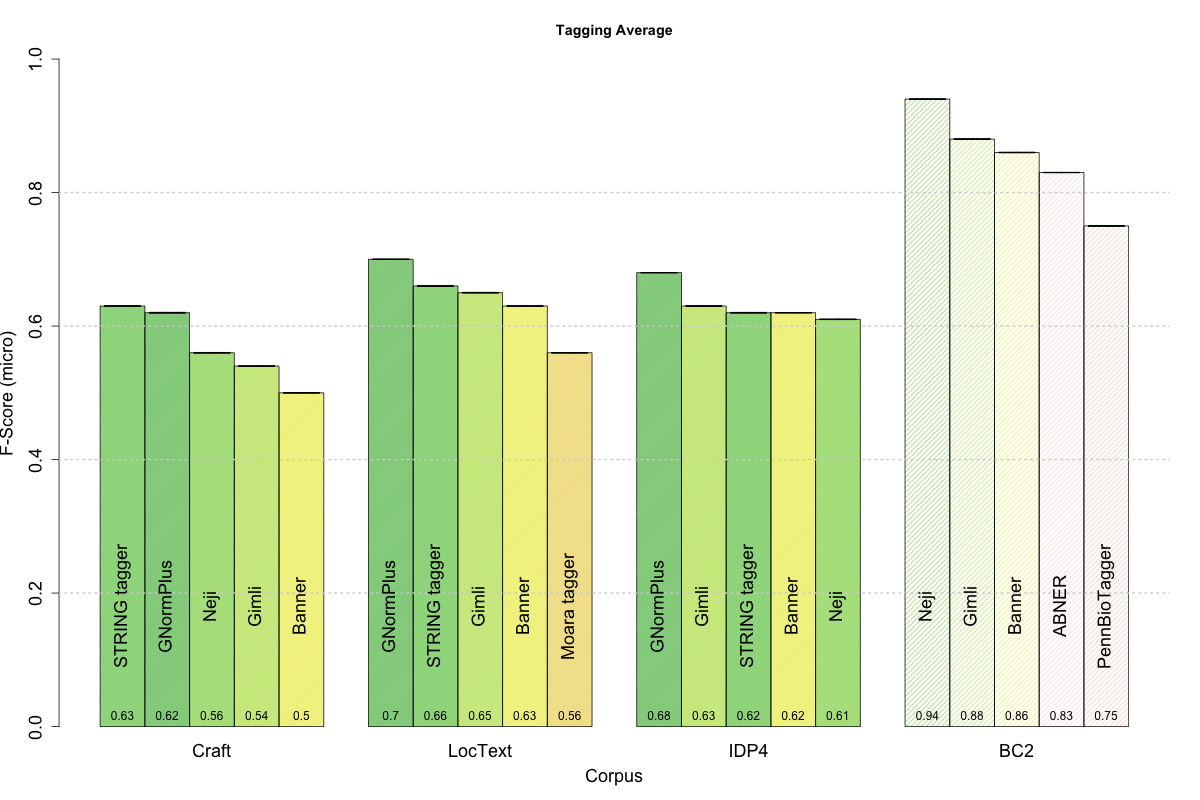
\includegraphics[width=5in]{Figures/eval/TaggingAverageOverview.png}
    \rule{35em}{0.5pt}
  \caption[Overview of the highest F-Scores in Average Tagging evaluation]{Overview of the highest F-Scores reached for Average Tagging evaluation on all evaluated corpora. Systems trained on the corpus used for evaluation are displayed in dashed colors. Standard errors are indicated for each F-Score, which appears as single sine due to very small span. Average  As the values of standard errors are very small, they appear as a single line. Adopted from (Ofner, 2015 \citep{ofner2015evaluation})}
  \label{fig:TaggingAverageFScore}
\end{figure}


\begin{figure}[htbp]
	\centering
    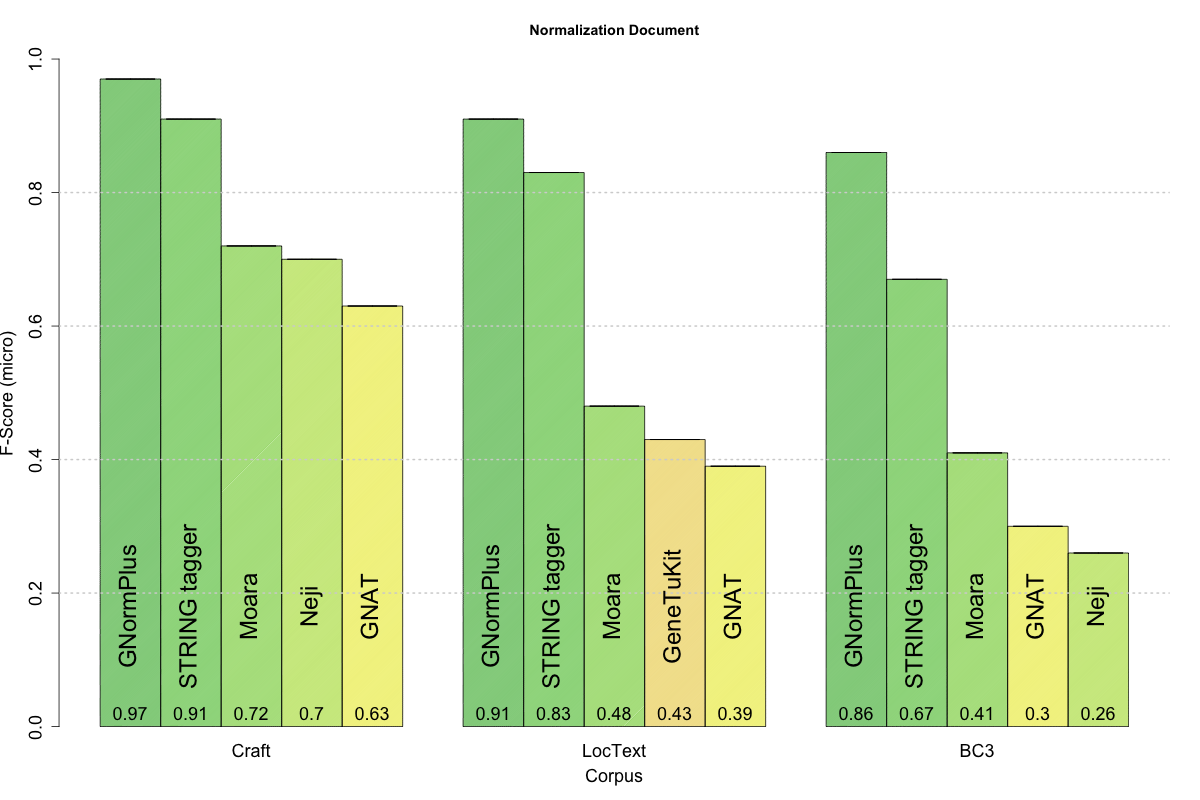
\includegraphics[width=3.5in]{Figures/eval/NormalizationDocumentOverview.png}
    \rule{35em}{0.5pt}
  \caption[Overview of the highest F-Scores in Document Level Normalization evaluation]{Overview of the highest F-Scores reached for Document Level Normalization evaluation on all evaluated corpora. Figure formatting follows \ref{fig:TaggingAverageFScore}. Adopted from (Ofner, 2015 \citep{ofner2015evaluation})}
  \label{fig:DocNormalizationFScore}
\end{figure}


\begin{figure}[htbp]
	\centering
    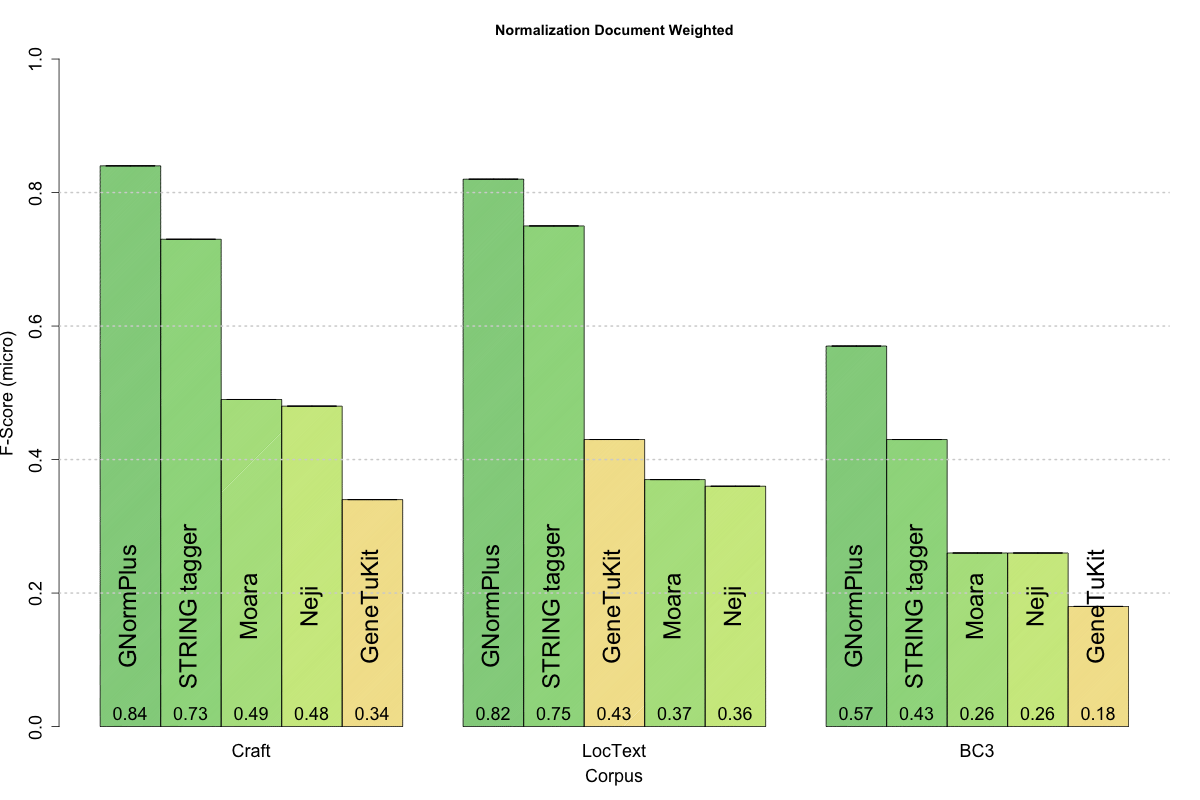
\includegraphics[width=3.5in]{Figures/eval/NormalizationDocumentWeightedOverview.png}
    \rule{35em}{0.5pt}
  \caption[Overview of the highest F-Scores in weighted Document Level Normalization evaluation]{Overview of the highest F-Scores reached for weighted Document Level Normalization evaluation on all evaluated corpora. Figure formatting follows \ref{fig:TaggingAverageFScore}. Adopted from (Ofner, 2015 \citep{ofner2015evaluation}).}
  \label{fig:AverageDocNormalizationFScore}
\end{figure}


\begin{figure}[htbp]
	\centering
    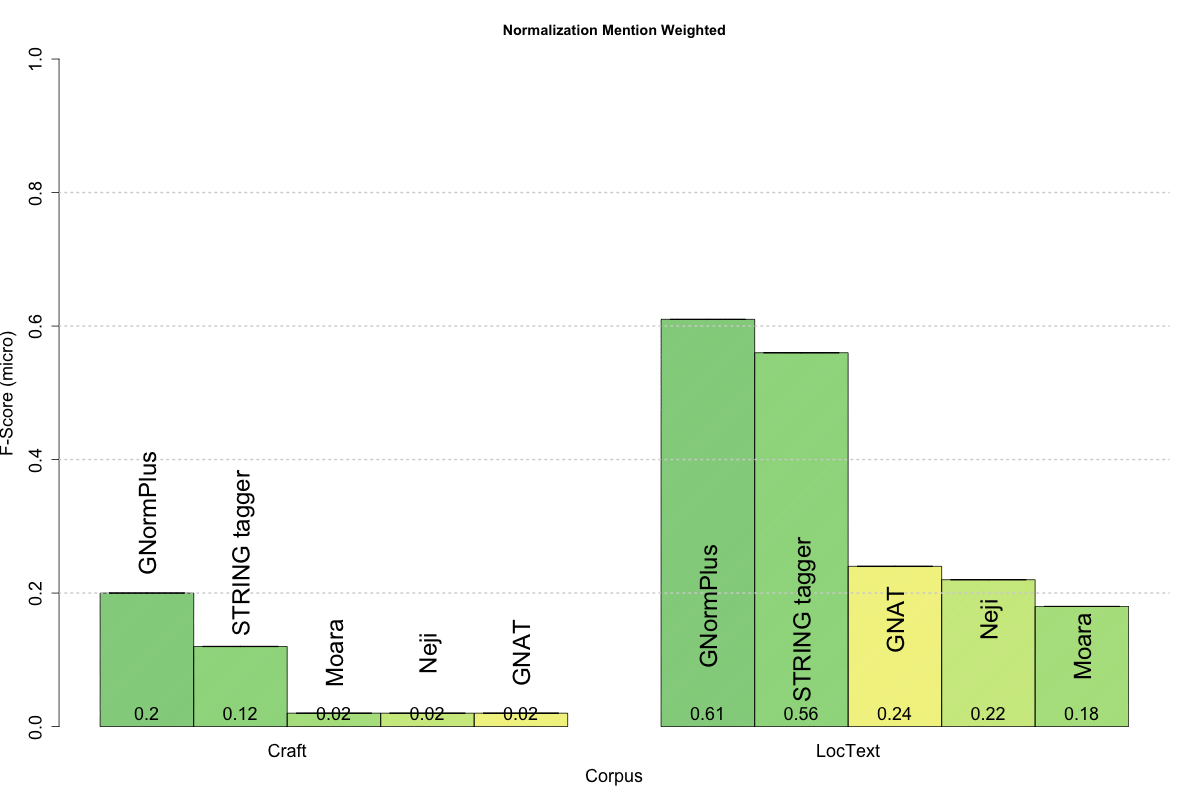
\includegraphics[width=3.5in]{Figures/eval/NormalizationMentionWeightedOverview.png}
    \rule{35em}{0.5pt}
  \caption[Overview of the highest F-Scores in Mention Normalization evaluation]{Overview of the highest F-Scores reached for Mention Normalization evaluation on all evaluated corpora. Figure formatting follows \ref{fig:TaggingAverageFScore}. Adopted from (Ofner, 2015 \citep{ofner2015evaluation}).}
  \label{fig:MentionNormalizationFScore}
\end{figure}

%----------------------------------------------------------------------------------------
%	SECTION 1
%----------------------------------------------------------------------------------------
\section{Tagging Pipeline}

As of writing of this thesis \footnote{31-08-2015}, we managed to index 24,770,062 unique MEDLINE references. This represents the whole body of MEDLINE at the time of writing. In the last 26 days, there were anywhere between 867 and 60726 new MEDLINE reference updates in a day (see Figure \ref{fig:NewArticles}). Note that not all of these MEDLINE references are new references. Several articles for example, contain errata and updates, which would be updated as a MEDLINE reference (with already existing PubMed ID). Figure shows the number of most commonly annotated species as of January 27. Note that the species count was done in singe-annotation basis. That is, three annotations from species \texttt{HUMAN} in an article would be considered as three counts.

\begin{figure}[htbp]
	\centering
    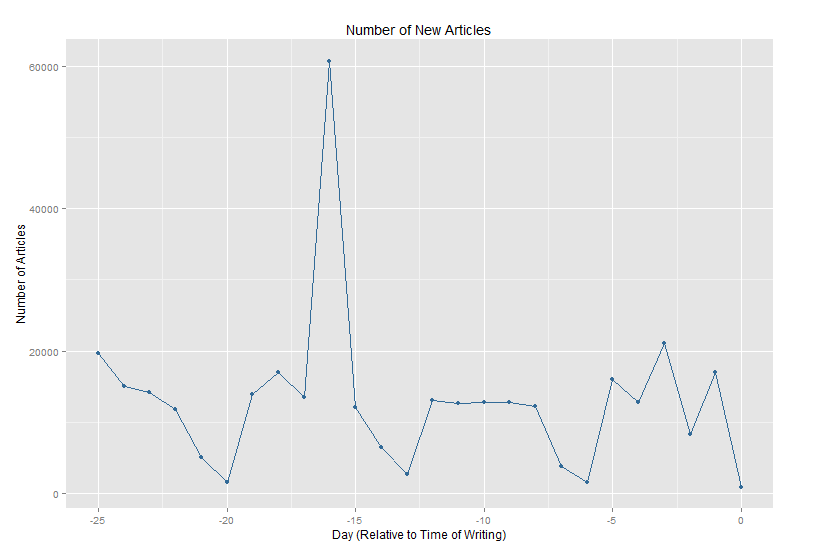
\includegraphics[width=6in]{Figures/NewArticles.png}
    \rule{35em}{0.5pt}
  \caption[Number of incoming MEDLINE updates]{Number of MEDLINE references that were updated every day from MEDLINE leasing scheme API in the last 26 days from the writing of the thesis (August 31, 2015). Note that not all of the references are new references. Some are for example erratas and updates.}
  \label{fig:NewArticles}
\end{figure}


\begin{table}[htbp]
\caption{Top 20 most annotated species in PubSeq. Note that UniProt species prefix of UniProt ID is used to create the statistics. The statistics shown is based on MEDLINE corpus dated January 27 2015.}
\centering
\begin{tabular}{ l c }
  \hline
  Species & Count \\
  \hline
  \hline
  \texttt{HUMAN} & 174234256 \\
  \hline
  \texttt{TRICA} & 10652136 \\
  \hline
  \texttt{PLAFA} & 3741883 \\
  \hline
  \texttt{AMPQE} & 2104511 \\
  \hline
  \texttt{MOUSE} & 1810839 \\
  \hline
  \texttt{ECOLX} & 1616597 \\
  \hline
  \texttt{YEASX} & 1148243 \\
  \hline
  \texttt{DROME} & 1064188 \\
  \hline
  \texttt{NEIME} & 697748 \\
  \hline
  \texttt{ARATH} & 602577 \\
  \hline
  \texttt{PlAVI} & 535429 \\
  \hline
  \texttt{RAT} & 376578 \\
  \hline
  \texttt{STREE} & 275870 \\
  \hline
  \texttt{KLEPN} & 259444 \\
  \hline
  \texttt{YEASK} & 214788 \\
  \hline
  \texttt{YEAS7} & 211277 \\
  \hline
  \texttt{YEAST} & 210358 \\
  \hline
  \texttt{STRPY} & 203976 \\
  \hline
  \texttt{YEAS6} & 200899 \\
  \hline
  \texttt{YEAS8} & 200899 \\
  \hline
\end{tabular}
  \label{tab:NERRanking}
\end{table}